\begin{flushright} {\tiny {\color{gray} benchmark\_laplace\_plate.tex}} \end{flushright}

This experiment is based on a 2nd year mathematics lecture I give at Utrecht University. 
One wishes to solve the Laplace equation for temperature on the following plate subject 
to the indicated boundary conditions:

\begin{center}
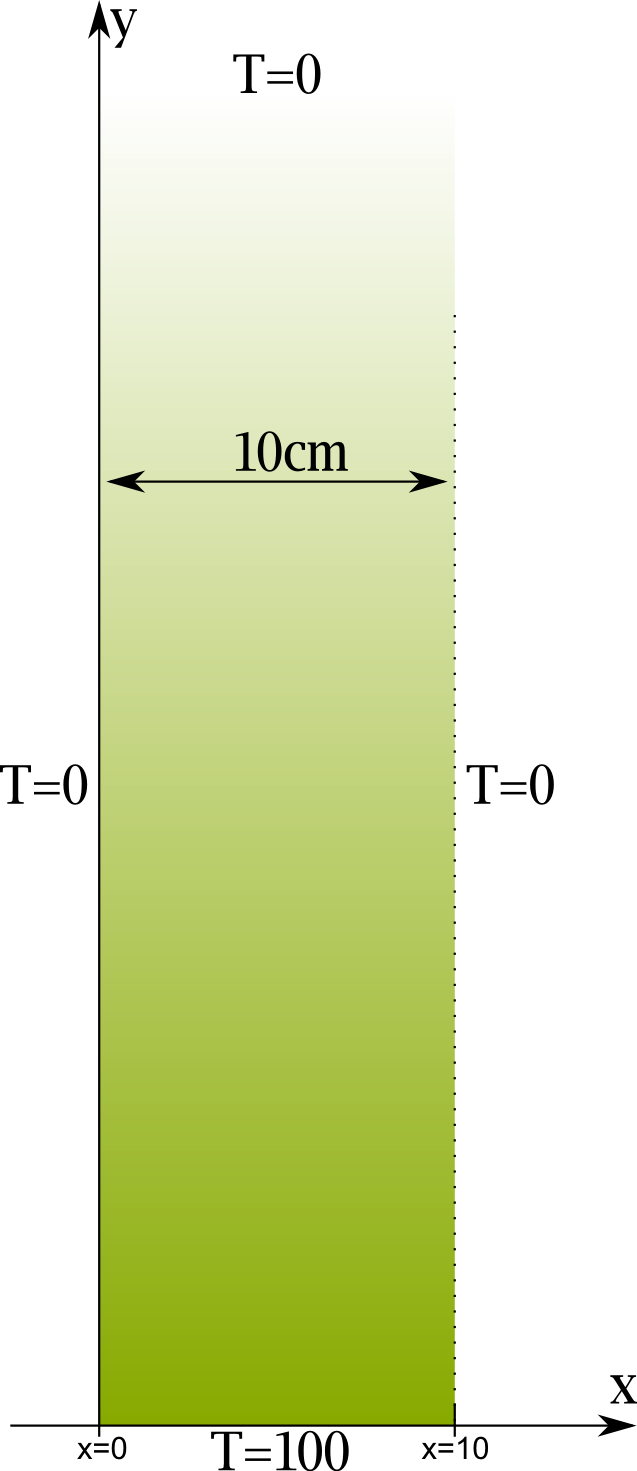
\includegraphics[width=3.5cm]{images/benchmark_lapplate/laplace2.png}
\end{center}


The temperature satisfies the 2D Laplace equation inside the plate:
\begin{equation}
\frac{\partial^2 T}{\partial x^2}
+ \frac{\partial^2 T}{\partial y^2} = 0
\end{equation}

We could try to solve the equation by using a tentative solution of the form:
\begin{equation}
T(x,y)=\theta(x) \Phi(y)
\end{equation}


\includegraphics[width=.5cm]{images/benchmark_lapplate/warning.png}
We do not {\it know} the solution is of this form.

We substitute (2) into (1) and obtain:
\[
\Phi \frac{\partial^2 \theta}{\partial x^2} +
\theta \frac{\partial^2 \Phi}{\partial y^2} = 0
\]
Dividing by $\theta\Phi$ gives:
\[
\frac{1}{\theta} \frac{\partial^2 \theta}{\partial x^2} +
\frac{1}{\Phi} \frac{\partial^2 \Phi}{\partial y^2} = 0
\]

Separation of variables: we say that each term is a constant because the first term is a function of $x$ only
and the second a function of $y$ only.
We then write
\[
\frac{1}{\theta} \frac{\partial^2 \theta}{\partial x^2} = - \frac{1}{\Phi} \frac{\partial^2 \Phi}{\partial y^2} = -k^2
\]
where $k$ is called the separation constant.
This leads to 
\[
\frac{\partial^2 \theta}{\partial x^2} + k^2 \theta = 0
\]
\[
\frac{\partial^2 \Phi}{\partial y^2} - k^2 \Phi =0
\]

\begin{itemize}
\item The solution to the first one is $\theta(x)=\sin kx$ or $\theta(x)=\cos kx$
\item The solution to the second one is $\Phi(x)=e^{kx}$ or $\Phi(x)=e^{-kx}$
\end{itemize}


The general solution writes:

\[
T(x,y)=\theta(x) \Phi(y)=
\left\{
\begin{array}{c}
\sin kx \\ \cos kx
\end{array}
\right\}
\left\{
\begin{array}{c}
e^{ky} \\ e^{-ky}
\end{array}
\right\}
\]

We can now use the b.c. to find the solution to the Laplace equation.

\begin{itemize}
\item Since $T\rightarrow 0$ when $y\rightarrow \infty$ then $e^{ky}$ unacceptable.
\item Since $T=0$ when $x=0$ then $\cos kx$ unacceptable.
\end{itemize}

so
\[
T(x,y)=
\sin (kx)  \;
 e^{-kx}
\]

We finally use $T=0$ at $x=10$ which leads to $10k=n \pi$, i.e.:

\[
T(x,y)=\sin (\frac{n\pi x}{10}) \;   e^{-n\pi y/10}
\]


\includegraphics[width=.5cm]{images/benchmark_lapplate/warning.png}
Problem: the solution does not satisfy  $T(x,0)=100$.
However, a linear combination of solutions is still a solution !
Let's find such a combination which satisfies the b.c. at $y=0$ :
\[
T(x,y) = \sum_{n=1}^\infty b_n \sin (\frac{n\pi x}{10}) \;   e^{-n\pi y/10}
\]

We impose then $T(x,0)=100$:
\[
100 = \sum_{n=1}^\infty b_n \sin (\frac{n\pi x}{10}) 
\]
This is the Fourier sine series of $f(x)=100$ with $l=10$ (chapter 7.9 of Boas).

The coefficient $b_n$ is then given by
\[
b_n=\frac{2}{l} \int_0^l f(x) \sin\frac{n \pi x}{l} dx
=\frac{2}{10} \int_0^l 100 \sin\frac{n \pi x}{10} dx
=
\left\{
\begin{array}{ll}
400/n\pi & {\rm odd \; n} \\
0 & {\rm even \; n} \\
\end{array}
\right.
\]

Finally (!):
\[
T(x,y) = 
\frac{400}{\pi}
\left(
e^{-\pi y/10} \sin (\frac{\pi x}{10})
+\frac{1}{3}
\sin (\frac{3\pi x}{10}) \;   e^{-3\pi y/10}
+ \dots
\right)
\]

The simulation has been run with a 10x50 domain. All coefficients of the temperature equation are
set to 1, and the Stokes equation is not solved. The timestep is fixed to $dt=0.1$. Resolution 
is 32x160. 

\begin{center}
a)

\includegraphics[width=1.8cm]{images/benchmark_lapplate/temper0000.png}
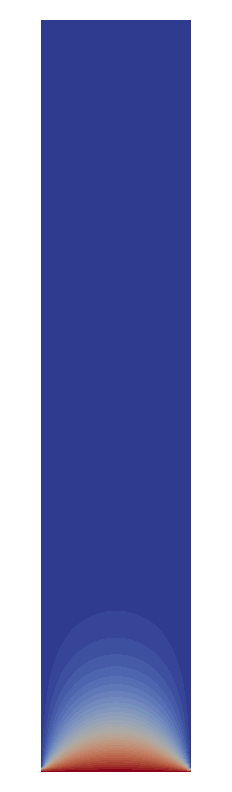
\includegraphics[width=1.8cm]{images/benchmark_lapplate/temper0010.png}
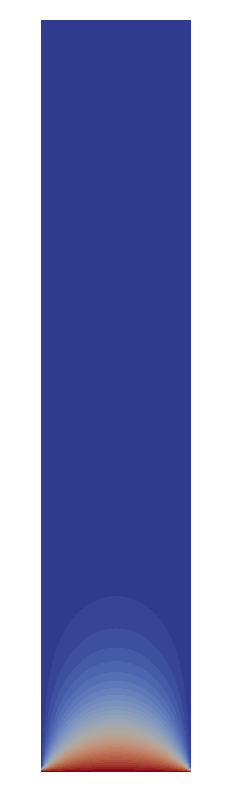
\includegraphics[width=1.8cm]{images/benchmark_lapplate/temper0020.png}
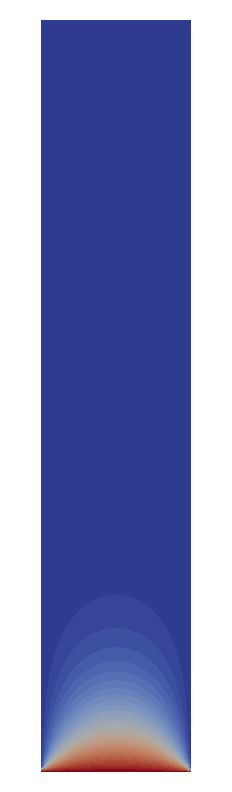
\includegraphics[width=1.8cm]{images/benchmark_lapplate/temper0030.png}
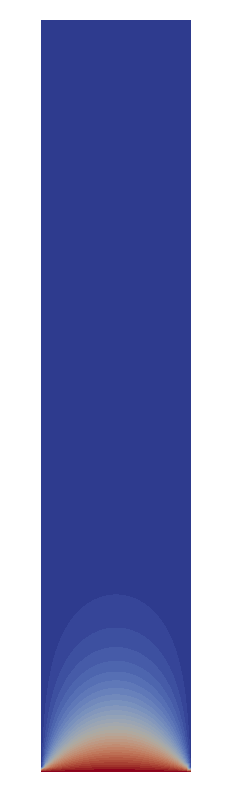
\includegraphics[width=1.8cm]{images/benchmark_lapplate/temper0040.png}
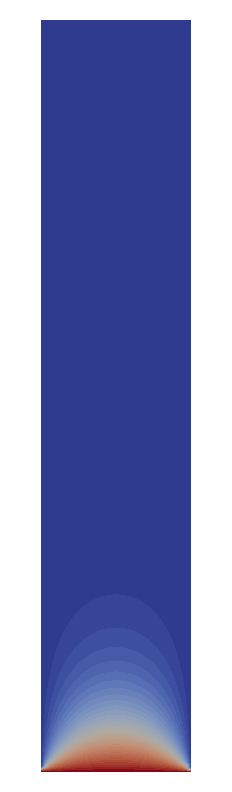
\includegraphics[width=1.8cm]{images/benchmark_lapplate/temper0050.png}
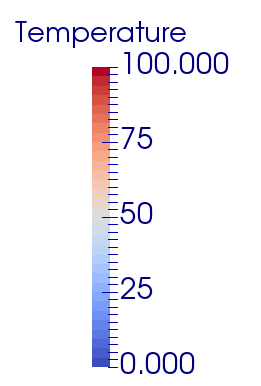
\includegraphics[width=1cm]{images/benchmark_lapplate/colourscale.png}
\hspace{.2cm}
b)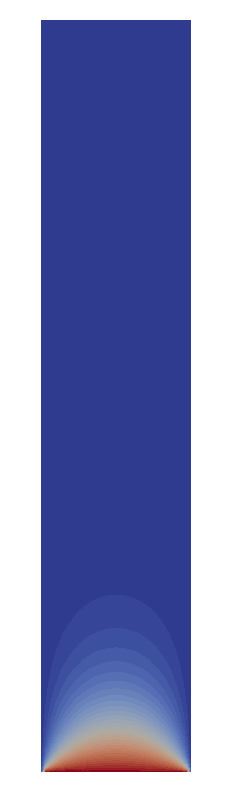
\includegraphics[width=1.8cm]{images/benchmark_lapplate/temper_analytical.png}\\
{\captionfont a) time evolution of the temperature field; b) analytical steady state solution}
\end{center}




